%27/10 - Paco Jurado
\chapter{Part-of-Speech (PoS) Tagging}
\section{Parts of Speech (PoS)}
El PoS tagging identifica las propiedades gramaticales de una palabra: nombres, verbos, adjetivos, etc. La ventaja es que hay clases cerradas (determinantes, preposiciones, pronombres, etc) y estandarizadas, aunque también hay algunas clases abiertas como nombres, verbos, adjetivos y adverbios. 

Penn Treebank contiene el tagset para inglés de forma estandarizada. Tiene la nomenclatura ya establecida, asignando el tag DT a los determinantes, FW a las palabras extranjeras, IN a las preposiciones, etc. 

Alternativamente está el conjunto Universal Dependencies (UD) que tiene 17 PoS tags en lugar de los 45 de Penn Treebank. Estos tags se agrupan en tres clases (abierto, cerrado y otro). 

\section{El problema del PoS tagging}
El etiquetado del PoS consiste en asignando a cada palabra o token de un texto su función dentro de la oración. A partir de ahí se podría hacer el análisis sintáctico, semántico e incluso del discurso. 

Algunas de las aplicaciones son:
\begin{itemize}
\item Reconocimiento de entidades: nombres propios, lugar, organización, persona
\item Desambigüación de palabras: diferentes significados de palabras pueden tener distintas clases.
\item Traducción
\item Análisis de opinión
\item Preguntas a respuestas
\item Sistemas de diálogos
\end{itemize}

El PoS tagging no es trivial, ya que una palabra puede tener una etiqueta distinta en función de su contexto. Esto ocurre mucho en inglés donde se adjetivan los verbos con -ing, aunque también pueden ser gerundios. La mayoría de las palabras del vocabulario no es ambigüo y se sabe exactamente lo que significa, pero el 14-15\% restante proporciona la ambigüedad al texto. 

Se puede optar por un baseline y coger la más frecuente, y esto da una precisión alta, del 92\%. Otros algoritmos llegan hasta el 97\% cuando se trata del inglés con algoritmos como HMM o campos aleatorios condicionales. Entre las diferentes aproximaciones hay léxicas, basadas en reglas (si una palabra termina en -ed o -ing, puede ser un verbo), probabilísticas (HMM y CRF) y basadas en redes neuronales.

\section{PoS tagging probabilístico}
\subsection{Modelos ocultos de Markov (HMM)}
Las cadenas de Markov son modelos estocásticos que describen las probabildiades de secuencias de variables aleatorias (estados). La probabilidad de cada evento depende solo del estado que se ha dado en el evento anterior. La probabilidad de cada evento depende solo del estado en el que estamos y del evento. 

Las cadenas ocultas tienen una serie de estados que van a venir de situaciones observables (cada uno de los tokens o palabras) y hay unos estados ocultos que son la función de cada token dentro de la oración (la etiqueta). Así, están los estados o procesos no observados (ocultos) y los procesos observables (palabras del texto). Hay dos asunciones: (1) La probabilidad de un estado concreto depende únicamente del estado anterior. (2) La probabilidad de una observación de salida depende únicamente del estado que produjo la observación y no de ningún otro estado ni de ninguna otra observación

La matriz de transición de probabilidades representa la probabilidad de pasar de una etiqueta a otra. Si tenemos un verbo modal, lo más seguro es que a continuación venga el verbo principal, no un sustantivo. Luego se estima la maximum likelihood. 

La matriz de emisión de probabilidades representa las probabilidades asociadas a cada palabra dada la etiqueta. Multiplicando las dos matrices se puede calcular la probabilidad de la etiqueta de una palabra. 

Así, el proceso tiene dos etapas:
\begin{enumerate}
\item Decoding: dado un input de HMM como secuencia de observaciones, se encuentran los estados más probables de la secuencia. 
\item Codificación para PoS tagging: se elige la secuencia de etiquetas que van a estar vinculados a lo que se observa. Como se trata de un modelo generador, si la primera etiqueta es un nombre propio, generamos un nombre propio con cierta probabilidad. Esto no lo utilizamos nosotros, si no que aplicamos la regla de Bayes para usar las matrices de probabilidad de generación para identificar. 
\end{enumerate}

En definitiva, hay un texto de entrenamiento con las etiquetas ya asignadas previamente (corpus etiquetado) que se utiliza con las probabilidades para asignar las etiquetas a un texto nuevo. Así, la probabilidad de que aparezca una palabra depende únicamente de su propia etiqueta, y es independiente de las palabras y etiquetas vecinas, y la probabilidad de una etiqueta depende únicamente de la etiqueta anterior, en lugar de toda la secuencia de etiquetas (supuesto del bigrama).

Para encontrar la secuencia de etiquetas que maximiza la probabilidad de Bayes, se utiliza el \textbf{algoritmo de Viterbi}. Es un algoritmo de programación dinámica que va buscando la secuencia más probable dada una serie de palabras. Mira todos los recorridos y luego las palabras. Coge la primera palabra y asigna su etiqueta, y busca los posibles caminos a continuación. Ve la siguiente palabra y confirma el camino correcto de las posibilidades, y calcula las siguientes ramificaciones. 

\begin{figure}[h]
\centering
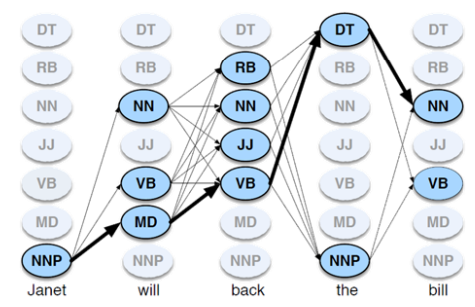
\includegraphics[width = 0.7\textwidth]{figs/viterbi.png}
\end{figure}

\subsection{Campos aleatorios condicionales (CRF)}
En los modelos ocultos de Markov, aprenden las etiquetas de un corpus para ahora generar etiquetas a un texto nuevo. Pero, ¿y si aparece una palabra que no estaba en el corpus? El algoritmo es fácil de implementar, pero es muy sensible cuando se altera el orden de las palabras y no haya aparecido al menos una vez en el corpus, ya que no se puede hacer la transición de los estados ocultos y no se va a reconocer como una secuencia válida. Aquí es donde entran los campos aleatorios condicionales.

Los campos aleatorios condicionales proporcionan resultados muy similares a las redes neuronales con menos maquinaria. No se utiliza un modelo generativo como en HMM, si no que se utiliza un modelo discriminativo. Se miran determinadas características de la palabra (por ejemplo, el lema y sufijos o prefijos, plurales, etc). Así, se buscan los atributos para cada palabra en una ventana de contexto específica (palabra + palabra anterior + palabra posterior, dos anteriores, dos posteriores, etc) y, en caso de que aparezca una palabra que no estaba en el corpus de entrenamiento, no pasa nada. Si acaba en -ed y tiene delante un nombre propio, con cierta probabilidad es un verbo porque se han visto patrones similares anteriormente, por lo que se etiqueta como tal. A través de las características se ve qué etiquetas no son y se discrimina así la etiqueta final. en HMM, se maximiza la probabilidad, y en CRF se discriminan todas las secuencias que maximizan la probabilidad.

Para cada palabra se define un modelo log-linear donde a cada uno de los atributos de la palabra se le asigna un peso. Aplicando unas fórmulas se llega a tener una probabilidad para la palabra. Se define una función que mapea las características de entrada a un determinado PoS tag. Se vuelve a aplicar el algoritmo de Viterbi, pero con las probabilidades calculadas a través de la CRF.

\section{PoS tagging basado en redes neuronales}
Los CRF siguen unas estructuras similares a perceptrones. Collins consiguió en 2012 una precisión del 97.1\% con Penn Tree utilizando un perceptron \footnote{Un perceptron es la red neuronal más simple. Recibe un input, realiza una transformación y saca un output. Si hay varias neuronas/perceptrones, se concatena.} estructurado y las características de current word, previous words, next words, previous tag y previous two tags, similar a las características empleadas en CRF.

\begin{figure}[h]
\centering
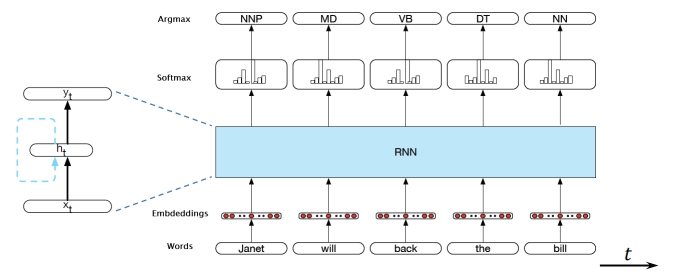
\includegraphics[width = 0.9\textwidth]{figs/rnn.png}
\caption{Red neuronal recurrente (RNN; recurrent neural network).}
\end{figure}

Entre una de las arquitecturas de las redes neuronales está la long short-term memory (LSTM). Es una red neuronal donde se van definiendo cómo están conectadas las neuronas y da un 95\% de precisión con CRF y 96.5\% con bi-LSTM (mira de izquierda a derecha y derecha a izquierda las palabras).